% Dit werk is gelicenseerd onder de licentie Creative Commons Naamsvermelding-GelijkDelen 4.0 Internationaal. Ga naar http://creativecommons.org/licenses/by-sa/4.0/ om een kopie van de licentie te kunnen lezen.
\chapter{Behoudsvergelijkingen voor controlevolumes}
\label{sec:Behoudsvergelijkingen voor controlevolumes}

%%%%%%%%%%%%%%%%%%%%%%%%%%%%%%%%%%%%%%%%%%%%%%%%%%%%%%%%%%%%%%%%%%%%%%%%%%%%%%%%%%
	\section{Inleiding}
	\label{sec:Controlevolume benadering Inleiding}
Wanneer een fluïdum in beweging is zullen belangrijke grootheden (drukken, krachten) niet enkel afhankelijk zijn van de eigenschappen van het fluïdum, maar ook afhankelijk zijn van de stroming. Deze stroming kunnen we beschrijven met behulp van het snelheidsveld. Veelal is dit snelheidsveld echter ook onbekend en zijn enkel de randvoorwaarden gekend. We hebben dus een manier nodig om het snelheidsveld te bepalen en hieruit de belangrijke grootheden te berekenen.

In dit hoofdstuk worden de begrippen controle massa en controlevolume geïntroduceerd. Een aantal behoudswetten worden afgeleid en er blijkt dat in sommige gevallen we voor het berekenen van grootheden uitgemiddeld over een volume of op de rand van het volume we enkel informatie over het snelheidsveld nodig hebben op de rand van het volume.

%%%%%%%%%%%%%%%%%%%%%%%%%%%%%%%%%%%%%%%%%%%%%%%%%%%%%%%%%%%%%%%%%%%%%%%%%%%%%%%%%%
	\section{Basis vergelijkingen voor controlemassa's}
	\label{sec:Basis vergelijkingen voor controlemassa's}
In de fysica en thermodynamica werden reeds een aantal natuurwetten geformuleerd. De vergelijkingen waar we in deze cursus gebruik van zullen maken zijn:
\begin{itemize}
	\item De wet van behoud van massa
	\item De tweede wet van Newton
	\item De wet van behoud van energie
\end{itemize}
De eerste is reeds geformuleerd als een behoudsvergelijking. Deze kan meteen geschreven worden als:
\begin{equation}
	\frac{\diff m}{\diff t} = 0
	\label{eqn:controlemassa,behoud van massa}
\end{equation}
De tweede wet van Newton kan ook als een behoudswet geformuleerd worden. Indien we het begrip \emph{impuls} invoeren als:
\begin{equation}
	\vt{P} = m\vt{v}
	\label{eqn:impuls}
\end{equation}
De tweede wet van Newton kan nu algemeen geschreven worden als de wet van behoud van impuls:
\begin{equation}
	\frac{\diff \vt{P}}{\diff t} = \vt{F}
	\label{eqn:controlemassa,behoud van impuls}
\end{equation}
De eerste hoofdwet van de thermodynamica is ook geformuleerd als een behoudsvergelijking, behoud van energie:
\begin{equation}
	\frac{\diff E}{\diff t} = \dot{Q}-\dot{W}
	\label{eqn:controlemassa,behoud van energie}
\end{equation}
Waarin $E$ de totale energie-inhoud van het systeem voorstelt, en $\dot{Q}$ en $\dot{W}$ respectievelijk de warmtestroom naar het systeem en het arbeidsvermogen uit het systeem voorstellen (stromen van een bepaalde grootheid zullen in deze cursus met een punt aangeduid worden).

Deze vergelijkingen zijn geformuleerd zodat ze geldig zijn voor een bepaald stelsel van deeltjes. 
De massa die in de eerste twee vergelijkingen voorkomt is dan de massa van de beschouwde deeltjes. De energie in de eerste hoofdwet is de energie inhoud van de beschouwde deeltjes. We noemen zo'n stelsel een systeem of een controlemassa.

Voor het gebruik in de fluïdummechanica zijn deze formuleringen echter niet zo geschikt. Een massa fluïdum zal namelijk steeds van vorm veranderen en kan zelfs opgesplitst worden in verschillende delen. Het uitwerken van de behoudswetten zal in de meeste gevallen niet eenvoudig zijn.

Het beschrijven van een fluïdumstroming is in de meeste gevallen eenvoudiger wanneer een deel van de ruimte wordt beschouwd waar het fluïdum door stroomt. Dit deel zal een bepaald volume in de ruimte innemen en wordt een \emph{controlevolume} genoemd.

De beschouwde behoudswetten zullen nu anders geformuleerd worden zodat ze toepasbaar zijn voor een controle volume.

%%%%%%%%%%%%%%%%%%%%%%%%%%%%%%%%%%%%%%%%%%%%%%%%%%%%%%%%%%%%%%%%%%%%%%%%%%%%%%%%%%
	\section{Basis vergelijkingen voor controlevolumes}
	\label{sec:Basis vergelijkingen voor controlevolumes}
In deze cursus zullen we de behoudswetten voor controlevolumes afleiden uit de behoudswetten voor controlemassa's door het extrapoleren van eenvoudige bevindingen. De behoudswetten kunnen ook rigoureus wiskundig afgeleid worden met behulp van het Reynolds transport theorema. Dit valt echter buiten het bereik van deze cursus. Geïnteresseerde lezers worden verwezen naar \cite{Schobeiri2010}.

			\subsection{Behoud van massa}
			\label{sec:Behoud van massa}
Om behoud van massa te herschrijven voor het gebruik in een controle volume beschouwen we een willekeurig controlevolume in een stroming (Figuur \ref{fig:controlevolume in stroming}). Wanneer er netto een bepaalde hoeveelheid massa het controlevolume uitstoomt zal de hoeveelheid massa binnen het controlevolume net zoveel afnemen. Op dezelfde manier is de som van de netto massastroom over de grens van het controlevolume naar buiten en de verandering van massa binnen het controlevolume gelijk aan nul.
\begin{figure}[htb]
	\centering
	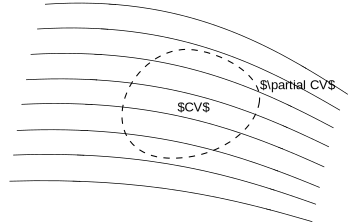
\includegraphics{fig/controlevolumes/Controlevolume_met_stroomlijnen}
	\caption{Willekeurig controlevolume in een stroming}
	\label{fig:controlevolume in stroming}
\end{figure}
\begin{equation}
	\left[
		\begin{array}{c}
			\mbox{De verandering} \\ \mbox{van massa in} \\ \mbox{het controlevolume}
		\end{array}
	\right]
	+
	\left[
		\begin{array}{c}
			\mbox{De netto} \\ \mbox{massastroom uit} \\ \mbox{het controlevolume}
		\end{array}
	\right]
	= 0
	\label{eqn:controlevolume,behoud van massa,woorden}
\end{equation}
In symbolen wordt dit:
\begin{equation}
	\frac{\diff m_{CV}}{\diff t} + \dot{m}_{\partial CV} = 0
	\label{eqn:controlevolume,behoud van massa}
\end{equation}
Deze vergelijking staat bekend als de wet van behoud van massa voor controlevolumes. Het subscript $CV$ staat in dit geval voor het controlevolume, het subscript $\partial CV$ staat voor de rand van het controlevolume.
Om de massastroom te evalueren beschouwen we een infinitesimaal klein oppervlak (Figuur \ref{fig:massastroom}).
\begin{figure}[htb]
	\centering
	\includegraphics{fig/controlevolumes/massastroom}
	\caption{Massastroom door een infinitesimaal oppervlak}
	\label{fig:massastroom}
\end{figure}
De hoeveelheid massa die in een tijdspanne $\Delta t$ door het oppervlak stroomt kan berekend worden als:
\begin{equation}
	\Delta m = \rho \Delta x_{\perp} \diff A = \rho v_{\perp} \Delta t \diff A
	\label{eqn:hoeveelheid massa door een oppervlak}
\end{equation}
Hierin is $v_{\perp}$ de loodrechte projectie van de snelheid op het oppervlak. De massastroom door het oppervlak $\diff A$ vinden we door te delen door de tijdspanne $\Delta t$:
\begin{equation}
	\diff \dot{m}  = \rho v_{\perp} \diff A
	\label{eqn:massastroom}
\end{equation}
Wanneer massastroom uit het controlevolume gericht is wordt de projectie van de snelheid positief gerekend, wanneer de massastroom het controlevolume in gericht is wordt de projectie negatief gerekend. Deze conventie komt overeen met de teken conventie van de vergelijking in woorden (\ref{eqn:controlevolume,behoud van massa,woorden}).

			\subsection{Behoud van impuls}
			\label{sec:Behoud van impuls}
Wanneer we de vergelijking van behoud van massa voor een controlevolume en een controle massa vergelijken zien we dat enkel het linker lid van vorm verandert. We kunnen dezelfde transformatie ook toepassen op de vergelijking van behoud van impuls. Dit wordt:
\begin{equation}
	\frac{\diff \vt{P}_{CV}}{\diff t} + \dot{\vt{P}}_{\partial CV} =  \vt{F}
	\label{eqn:controlevolume,behoud van impuls}
\end{equation}
In woorden wordt dit:
\begin{equation}
	\left[
		\begin{array}{c}
			\mbox{De verandering} \\ \mbox{van impuls in} \\ \mbox{het controlevolume}
		\end{array}
	\right]
	+
	\left[
		\begin{array}{c}
			\mbox{De netto} \\ \mbox{impulsstroom uit} \\ \mbox{het controlevolume}
		\end{array}
	\right]
	=
	\left[
		\begin{array}{c}
			\mbox{De totale} \\ \mbox{kracht op het} \\ \mbox{controlevolume}
		\end{array}
	\right]
	\label{eqn:controlevolume,behoud van impuls,woorden}
\end{equation}
De impulsstroom door een infinitesimaal oppervlak $\diff A$ kan als volgt berekend worden:
\begin{equation}
	\diff \dot{\vt{P}} =  \diff \dot{m} \vt{v} = \rho v_{\perp} \vt{v} \diff A
	\label{eqn:impulsstroom}
\end{equation}
Deze vergelijking is net zoals de impulsvergelijking voor controlemassa's een vectorvergelijking en kan dus geprojecteerd in een gewenste richting.

De term, de totale kracht op het controlevolume, zorgt soms voor verwarring. Krachten kunnen inwerken op een controlevolume via drukspanningen (normaalspanningen) en schuifspanningen. Wanneer de rand van een controlevolume tegen een wand valt zullen deze spanningen uitgeoefend worden door de wand en zal de wand gelijke maar tegengestelde reactie spanningen ondervinden. Deze spanningen kunnen dan voorgesteld worden als een resulterende reactiekracht. Wanneer de rand van het controlevolume in het medium valt zullen ook hier spanningen uitgeoefend worden door het medium buiten het controlevolume. De meest voor de hand liggende spanning is een drukspanning die gelijk in alle richtingen aanwezig is in het medium dus ook aan de rand van het controlevolume.


			\subsection{Behoud van energie}
			\label{sec:Behoud van energie}
Ook voor behoud van energie kunnen we dezelfde transformatie als voor massa en impuls toepassen. (\ref{eqn:controlemassa,behoud van energie}) wordt dan:
\begin{equation}
	\frac{\diff E_{CV}}{\diff t} + \dot{E}_{\partial CV} =  \dot{Q}-\dot{W}
	\label{eqn:controlevolume,behoud van energie}
\end{equation}
In woorden wordt dit:
\begin{equation}
	\left[
		\begin{array}{c}
			\mbox{De verandering} \\ \mbox{van energie in} \\ \mbox{het controlevolume}
		\end{array}
	\right]
	+
	\left[
		\begin{array}{c}
			\mbox{De netto} \\ \mbox{energiestroom uit} \\ \mbox{het controlevolume}
		\end{array}
	\right]
	=
	\left[
		\begin{array}{c}
			\mbox{De warmtestroom toegevoegd} \\ \mbox{en arbeidsstroom onttrokken} \\ \mbox{aan het controlevolume}
		\end{array}
	\right]
	\label{eqn:controlevolume,behoud van energie,woorden}
\end{equation}

%%%%%%%%%%%%%%%%%%%%%%%%%%%%%%%%%%%%%%%%%%%%%%%%%%%%%%%%%%%%%%%%%%%%%%%%%%%%%%%%%%
	\section{Stationair controlevolume met één instroming en één uitstroming}	
Bij ingenieurstoepassingen komt het vaak voor dat we controlevolumes beschouwen met slechts één instroming en één uitstroming. Voorbeelden zijn een simpele leiding, een pomp of turbine, een reactorvat,... 
Figuur \ref{fig:controlevolume een in en uitstroming} geeft een schematische voorstelling van zo'n situatie met bijhorend controlevolume. Het controlevolume is hier net tegen de wand van het systeem gekozen. Dit heeft als groot voordeel dat de projectie van de snelheid op de normaalvector enkel aan de instroom en de uitstroom verschillend is van nul. Aan de overige randen van het controlevolume kan er enkel een snelheid tangentieel aan de wand bestaan. De loodrechte component van de snelheid is dus $0$.
\begin{figure}[htb]
	\centering
	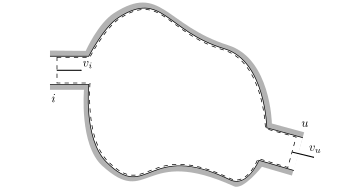
\includegraphics{fig/controlevolumes/Controlevolume_een_in_en_uitstroming}
	\caption{Controlevolume met één instroming en één uitstroming}
	\label{fig:controlevolume een in en uitstroming}
\end{figure}
De vergelijking voor behoud van massa (\ref{eqn:controlevolume,behoud van massa}) kunnen we schrijven als:
\begin{equation}
	\dfrac{\diff m_{CV}}{\diff t} + \dot{m}_{u} - \dot{m}_{i} = 0
	\label{eqn:behoud van massa in een controlevolume met een in en uitstroming}
\end{equation}
Dit kunnen we verder uitwerken door het massadebiet te berekenen als  het gemiddelde van de dichtheid maal de loodrechte snelheid maal het oppervlak. Wanneer we ook de gemiddelde dichtheid over de in en uitlaatsecties kennen, kunnen we (\ref{eqn:behoud van massa in een controlevolume met een in en uitstroming}) schrijven als:
\begin{equation}
	\dfrac{\diff m_{CV}}{\diff t} + \rho_{u} v_{u,\perp} A_{u} - \rho_{i} v_{i,\perp} A_{i} = 0
	\label{eqn:behoud van massa in een controlevolume met een in en uitstroming2}
\end{equation}
Wanneer daarbovenop we een stationaire situatie beschouwen, wordt de tijdsafgeleide in (\ref{eqn:behoud van massa in een controlevolume met een in en uitstroming2}) $0$:
\begin{equation}
	\rho_i v_{i,\perp} A_i = \rho_u v_{u,\perp} A_u
	\label{eqn:behoud van massa in een stationair controlevolume met een in en uitstroming}
\end{equation}
Bovenstaande vergelijking zegt dus niets anders dan dat het ingaande massadebiet gelijk is aan het uitgaande massadebiet. Dezelfde uitdrukking is ook geldig voor een niet-stationaire, niet-samendrukbare stroming door een controlevolume waarvan het volume constant is. Bijvoorbeeld een niet-stationaire stroming van water bij een lage snelheid door een stalen buis.

Passen we nu behoud van impuls toe op hetzelfde controlevolume uit Figuur \ref{fig:controlevolume een in en uitstroming}. We kunnen opnieuw gebruik maken van de gemiddelde eigenschappen bij de in en uitstroming.
\begin{equation}
	 \dfrac{\diff m \vt{v}_{CV}}{\diff t} + \rho_{u} v_{u,\perp} \vt{v}_{u} A_{u} - \rho_{i} v_{i,\perp} \vt{v}_{i} A_{i} = \vt{F}
	\label{eqn:behoud van impuls in een controlevolume met een in en uitstroming}
\end{equation}
In de tweede en derde term van bovenstaande vergelijking staat telkens de combinatie $\rho v_{\perp} A$ die gelijk is aan het massadebiet. Voor een stationaire stroming kunnen we (\ref{eqn:behoud van impuls in een controlevolume met een in en uitstroming}) dus verder vereenvoudigen aangezien ook hier de tijdsafgeleide $0$ wordt:
\begin{equation}
	\dot{m} (\vt{v}_u-\vt{v}_i) = \vt{F}
	\label{eqn:behoud van impuls in een stationair controlevolume met een in en uitstroming}
\end{equation}
Let wel, de krachten en snelheden voorkomend in deze vergelijking zijn vectoren, de vergelijking is dus een vectorvergelijking en kan geprojecteerd worden in verschillende richtingen. Als voorbeeld wordt (\ref{eqn:behoud van impuls in een stationair controlevolume met een in en uitstroming}) geprojecteerd op de assen van een cartesiaans assenstelsel. We bekomen:
\begin{align}
	F_x &= \dot{m} (v_{x,u}-v_{x,i}) \nonumber \\
	F_y &= \dot{m} (v_{y,u}-v_{y,i}) \\
	F_z &= \dot{m} (v_{z,u}-v_{z,i}) \nonumber
	\label{eqn:behoud van impuls in een stationair controlevolume met een in en uitstroming geprojecteerd}
\end{align}
Voor het bepalen van de inwerkende krachten moet ook hier rekening gehouden worden met de krachten aan de instroming en de uitstroming. De aan de instroming heersende druk zal namelijk een kracht $\vt{F} = - p A \vt{n}$ uitoefenen op het controlevolume met $\vt{n}$ de naar buiten gerichte normaalvector op de rand van het controle volume:
\begin{align}
	F_{x,R} &= p_{u} A_u n_{x,u} + p_{i} A_i n_{x,i} + \dot{m} (v_{x,u}-v_{x,i}) \nonumber \\
	F_{y,R} &= p_{u} A_u n_{y,u} + p_{i} A_i n_{y,i} + \dot{m} (v_{y,u}-v_{y,i}) \\
	F_{z,R} &= p_{u} A_u n_{z,u} + p_{i} A_i n_{z,i} + \dot{m} (v_{z,u}-v_{z,i}) \nonumber
	\label{eqn:behoud van impuls in een stationair controlevolume met een in en uitstroming geprojecteerd2}
\end{align}

We kunnen ook behoud van energie toepassen op het beschouwde controlevolume. De energie kunnen we opsplitsen in inwendige, kinetische en potentiële energie. Deze kunnen we op hun beurt schrijven als de gemiddelde waarde van de specifieke grootheden vermenigvuldigd met de massa:
\begin{equation}
	E = E_{inwendig} + E_{kinetisch} + E_{potenieel} = m u + m \frac{1}{2}v^2 + m g z
\end{equation}
Behoud van energie in een het stationair controlevolume wordt dan:
\begin{equation}
	\rho_{u} v_{u,\perp} (u_u + \frac{1}{2}v^2_u + g z_u) A_{u} - \rho_{i} v_{i,\perp} (u_i + \frac{1}{2}v^2_i + g z_i) A_{i} = \dot{Q}-\dot{W}
	\label{eqn:behoud van energie in een controlevolume met een in en uitstroming}
\end{equation}
Wanneer we de ingang en de uitgang naderbij bestuderen zien we dat hier arbeid wordt uitgeoefend op het controlevolume. Dit kunnen we eenvoudig inzien indien we een controlemassa beschouwen die zich aan de uitgang, net buiten het controlevolume bevindt (Figuur \ref{fig:stromingsarbeid}). Aangezien aan de uitgang een bepaalde druk heerst zal op de controlemassa een kracht worden uitgeoefend door het controlevolume. En aangezien de massa met de uitgaande snelheid beweegt wordt er dus een vermogen onttrokken aan het controlevolume. Aan de ingang kan een analoge redenering gevolgd worden.
\begin{figure}[htb]
	\centering
	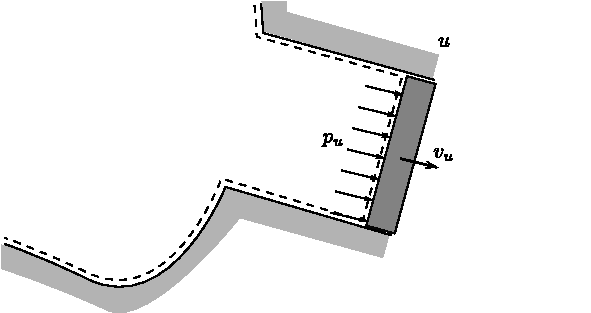
\includegraphics{fig/controlevolumes/Controlevolume_stromingsarbeid}
	\caption{Uitgang van een controlevolume met een aangrenzende controlemassa}
	\label{fig:stromingsarbeid}
\end{figure}
We kunnen dus de arbeidsvermogen uitgeoefend door het controlevolume op de omgeving opsplitsen in twee delen. Een eerste deel bestaat uit het vermogen geleverd aan de stroming aan de in en uitgangen. Dit noemen we de stromingsarbeid. Het overige vermogen zal uitgeoefend worden op bijvoorbeeld een schoepenrij in het controlevolume. Dit deel zal meestal omgevormd worden naar een mechanisch vermogen op een as, het wordt dan ook asvermogen genoemd.
\begin{equation}
	\dot{W} = \dot{W}_s + \dot{W}_a
	\label{eqn:stromings en asvermogen}
\end{equation}
Het stromingsvermogen kunnen we uitwerken als de uitgeoefende kracht vermenigvuldigd met de snelheid van de stroming aan de in en uitgangen. Met in acht name van de tekenconventie wordt dit:
\begin{equation}
	\dot{W}_s = p_u A_u v_u - p_i A_i v_i
	\label{eqn:stromingsvermogen}
\end{equation}
Wanneer we (\ref{eqn:stromings en asvermogen}) en (\ref{eqn:stromingsvermogen}) invullen in (\ref{eqn:behoud van energie in een controlevolume met een in en uitstroming}) bekomen we na omvorming en invullen van het massadebiet:
\begin{equation}
	\dot{m} (u_u + \frac{p_u}{\rho_u} + \frac{1}{2}v^2_u + g z_u) - \dot{m} (u_i + \frac{p_i}{\rho_i}+ \frac{1}{2}v^2_i + g z_i) = \dot{Q}-\dot{W}_a
	\label{eqn:behoud van energie in een controlevolume met een in en uitstroming asvermogen}
\end{equation}
De termen $u + \frac{p}{\rho}$ kennen we reeds uit de thermodynamica als de enthalpie $h$.

\begin{voorbeeld}
	Bereken de axiale en tangentiële kracht die uitgeoefend wordt op één schoep van de stilstaande schoepenrij in onderstaande figuur met hoogte $h$, de afstand tussen 2 schoepen is $b$. Door de schoepenrij stroomt een fluïdum met dichtheid $\rho$, voor de schoepenrij is verloopt de stroming axiaal en is de snelheid $v_{in}$. Na de schoepenrij maak en de stroomlijnen een hoek $\alpha$ met de axiale richting en is de druk $p_{uit}$. De stroming is stationair en adiabatisch en er zijn geen energieverliezen.
	\begin{center}
		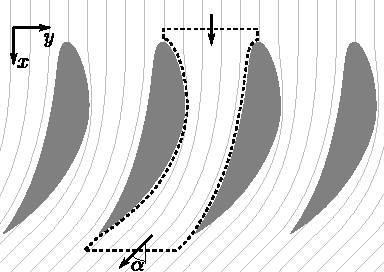
\includegraphics{fig/controlevolumes/Schoepenrij}
	\end{center}

	Beginnen de analyse door een geschikt controlevolume te tekenen zoals aangeduid in de figuur. Het controle volume loopt volgens de stroomlijnen tussen twee schoepen door en wordt afgsloten door twee vlakken volgens de tangentiële richting. Definieer ook een geschikt assenstelsel.

	Om de krachten uit te rekenen kunnen we de vergelijking van behoud van impuls uitschrijven voor het controlevolume. Aangezien dit volgens de stoomlijnen loopt hebben we een controlevolume met één inlaat en één uitlaat. Behoud van impuls wordt dan:
	\begin{align*}
		\sum F_x &= \dot{m} \left(v_{uit,x} - v_{in,x}\right) \\
		\sum F_y &= \dot{m} \left(v_{uit,y} - v_{in,y}\right)
	\end{align*}

	De snelheidscomponenten kunnen we halen uit de vergelijkingen voor behoud van massa. dit geeft:
	\begin{equation*}
		\rho v_{in} b h = \rho v_{uit} b h \cos \alpha
	\end{equation*}
	of:
	\begin{equation*}
		v_{uit} = \frac{v_{in}}{\cos \alpha}
	\end{equation*}
	dus:
	\begin{align*}
		v_{in,x}  &= v_{in}\\
		v_{uit,x} &= v_{in}\\
		v_{in,y}  &= 0\\
		v_{uit,y} &= -v_{in}\tan \alpha
	\end{align*}
	Het massadebiet halen we uit de doorstroom oppervlakte en de ingaande snelheid:
	\begin{equation*}
		\dot{m} = \rho b h v_{in}
	\end{equation*}

	Bovenstaande uitdrukkingen invullen geeft:
	\begin{align*}
		\sum F_x &= 0 \\
		\sum F_y &= -\rho b h v_{in}^2 \tan \alpha
	\end{align*}

	In de $x$-richting worden er krachten op het controlevolume uitgeoefend door de druk aan de boven en onderzijde van het controle volume en door de schoepen:
	\begin{equation*}
		\sum F_x = p_{in} b h - p_{uit} b h - F_{schoep,x}
	\end{equation*}
	In de $y$ richting wordt er enkel door de schoepen een kracht uitgeoefend, de druk krachten links en rechts heffen elkaar op.
	\begin{equation*}
		\sum F_y = - F_{schoep,y}
	\end{equation*}
	Door het min teken in te voeren bij de schoepkrachten stellen deze de kracht voor die de stroming uitoefent op de schoep, zoals gevraagd. In de vergelijking voor behoud van impuls staat namelijk de kracht die op het controlevolume wordt uitgeoefend.

	Om de druk voor de schoepenrij te berekenen kunnen we behoud van energie toepassen. Aangezien er geen verliezen zijn en de stroming adiabatisch verloopt is er geen toegevoegde warmte of onttrokken arbeid en blijft de inwendige energie constant:
	\begin{equation*}
		\dot{m} \left(\frac{p_{uit}}{\rho} + \frac{1}{2}v^2_{uit}\right) - \dot{m} \left(\frac{p_{in}}{\rho}+ \frac{1}{2}v^2_{in} \right) = 0
	\end{equation*}
	of:
	\begin{align*}
		 p_{uit} - p_{in} &= \frac{1}{2} \rho \left(v^2_{in} - v^2_{uit} \right) \\
		                  &= \frac{1}{2} \rho v^2_{in} \left(1 - \frac{1}{\cos^2 \alpha} \right) \\
		                  &= \frac{1}{2} \rho v^2_{in} \tan^2 \alpha
	\end{align*}

	Met deze uitdrukkingen kunnen we de schoepkrachten uitrekenen als:
	\begin{align*}
		F_{schoep,x} &= \rho b h  v^2_{in} \frac{1}{2} \tan^2 \alpha \\
		F_{schoep,y} &= \rho b h v_{in}^2 \tan \alpha
	\end{align*}
\end{voorbeeld}
